\documentclass[a4paper,11pt]{article}
\usepackage{amsmath,amsthm,amssymb}
\usepackage[utf8]{inputenc}
\usepackage[english,russian]{babel}
\usepackage[export]{adjustbox}
\usepackage{graphicx}
\usepackage{pgfplots}
\usepackage{textcomp}

\graphicspath{{pictures/}}
\DeclareGraphicsExtensions{.pdf,.png,.jpg}
\leftskip=-0cm 
\rightskip=-0cm
\voffset = -3cm
\hoffset = -3cm
\textwidth = 550pt
\textheight = 770pt
\pgfplotsset{width=10cm,compat=1.9}


\begin{document}
\Large
HW9
\\
1

\begin{center}
\center{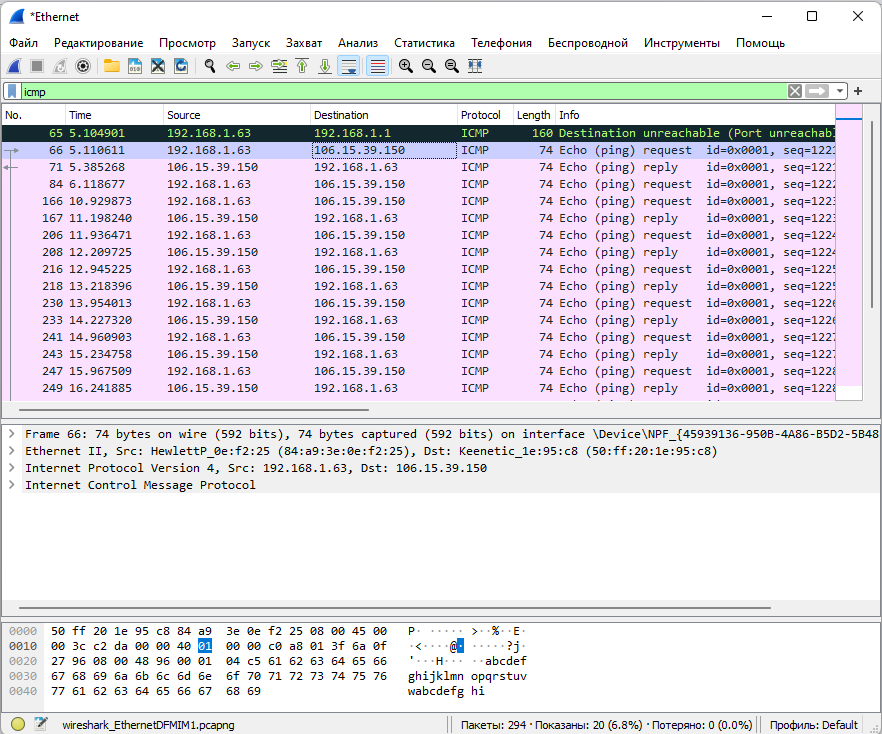
\includegraphics[width =\textwidth]{screenshots/1.png}}
\label{fig:image}
\end{center}
1) Мой IP 192.168.1.63

Адрес назначения	106.15.39.150

2) Так как ICMP - сетевой уровень, а порты на транспортном


\begin{center}
\center{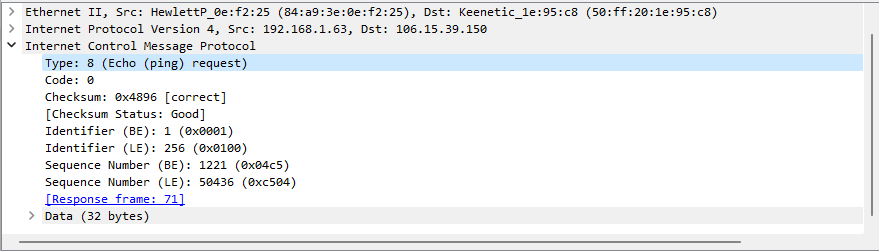
\includegraphics[width =\textwidth]{screenshots/2.png}}
\label{fig:image}
\end{center}
3) Type: 8 (Echo (ping) request)

Code: 0

Checksum: 0x4896 [correct]

Identifier (BE): 1 (0x0001)

Identifier (LE): 256 (0x0100)

Sequence Number (BE): 1221 (0x04c5)

Sequence Number (LE): 50436 (0xc504)

Поля по 2 байта

\begin{center}
\center{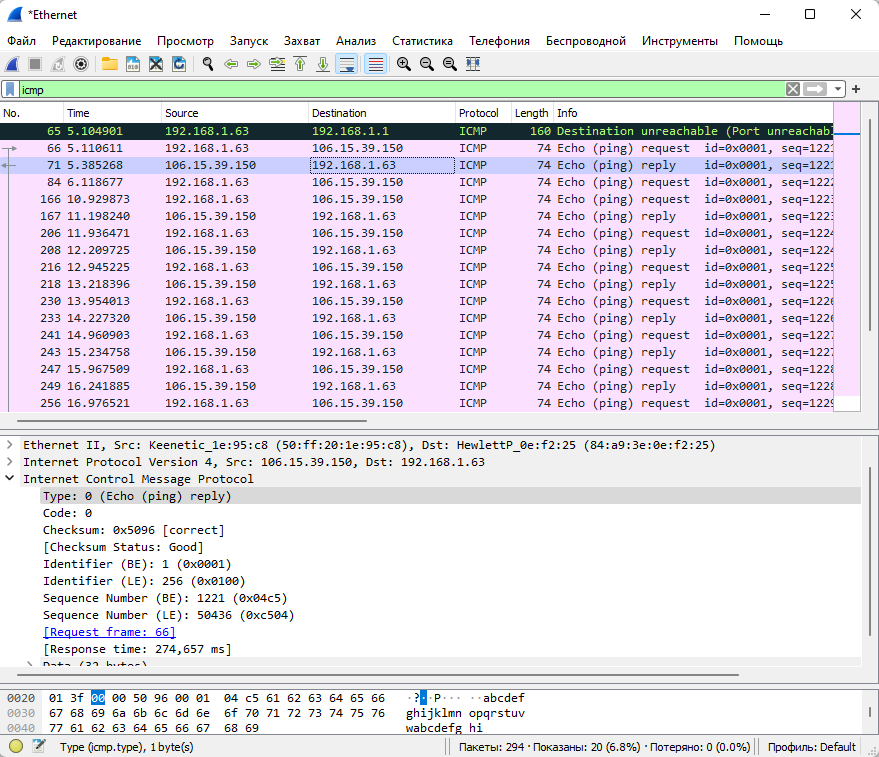
\includegraphics[width =0.95\textwidth]{screenshots/3.png}}
\label{fig:image}
\end{center}
4) Type: 0 (Echo (ping) reply)

Code: 0

Checksum: 0x5096 [correct]

Identifier (BE): 1 (0x0001)

Identifier (LE): 256 (0x0100)

Sequence Number (BE): 1221 (0x04c5)

Sequence Number (LE): 50436 (0xc504)

Поля по 2 байта
\newpage
2

\begin{center}
\center{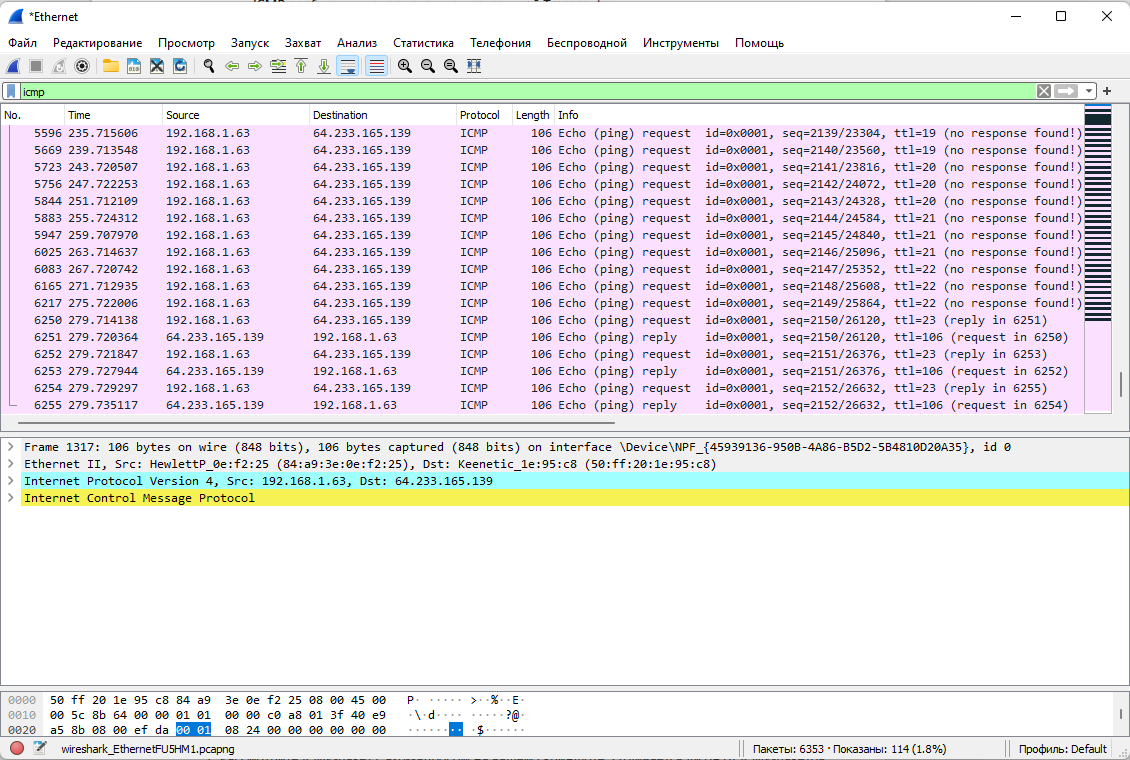
\includegraphics[width =0.95\textwidth]{screenshots/4.png}}
\label{fig:image}
\end{center}

\begin{center}
\center{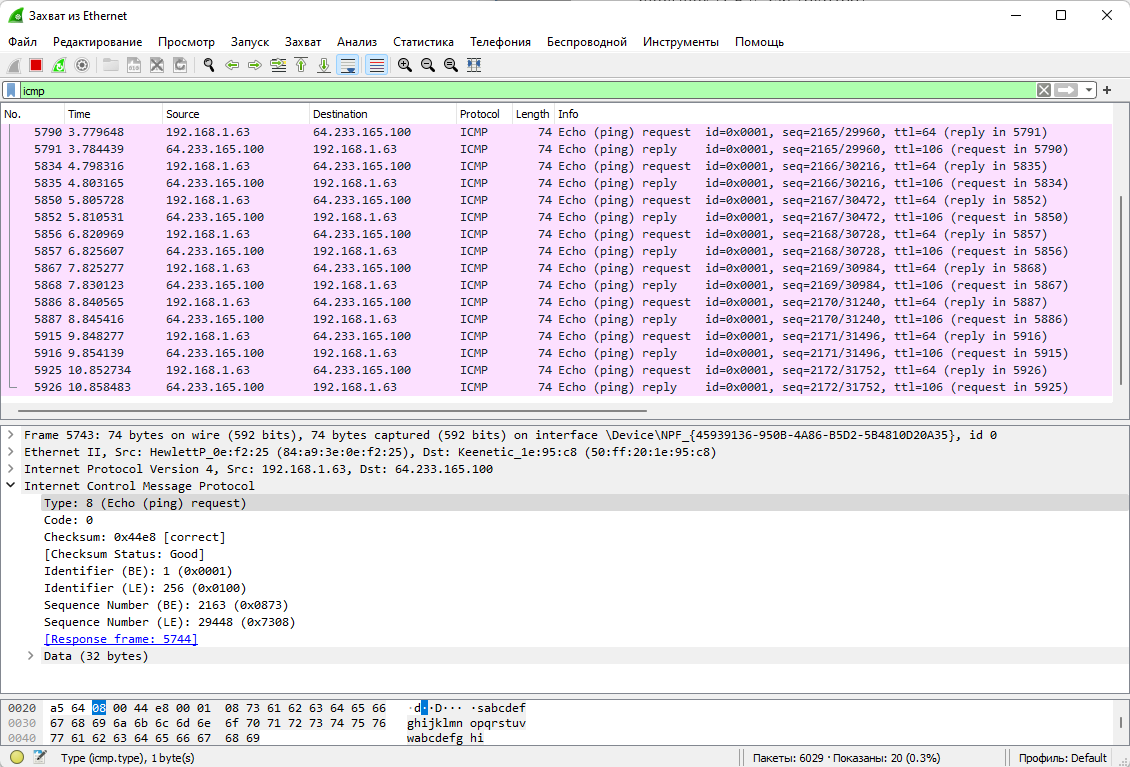
\includegraphics[width =0.95\textwidth]{screenshots/9.png}}
\label{fig:image}
\end{center}
1) Отличие в поле TTL (ping фиксированное 64 (в ответе 106), tracert от 1 до 23), размер data (32 ping, 64 tracert).

2)
\begin{center}
\center{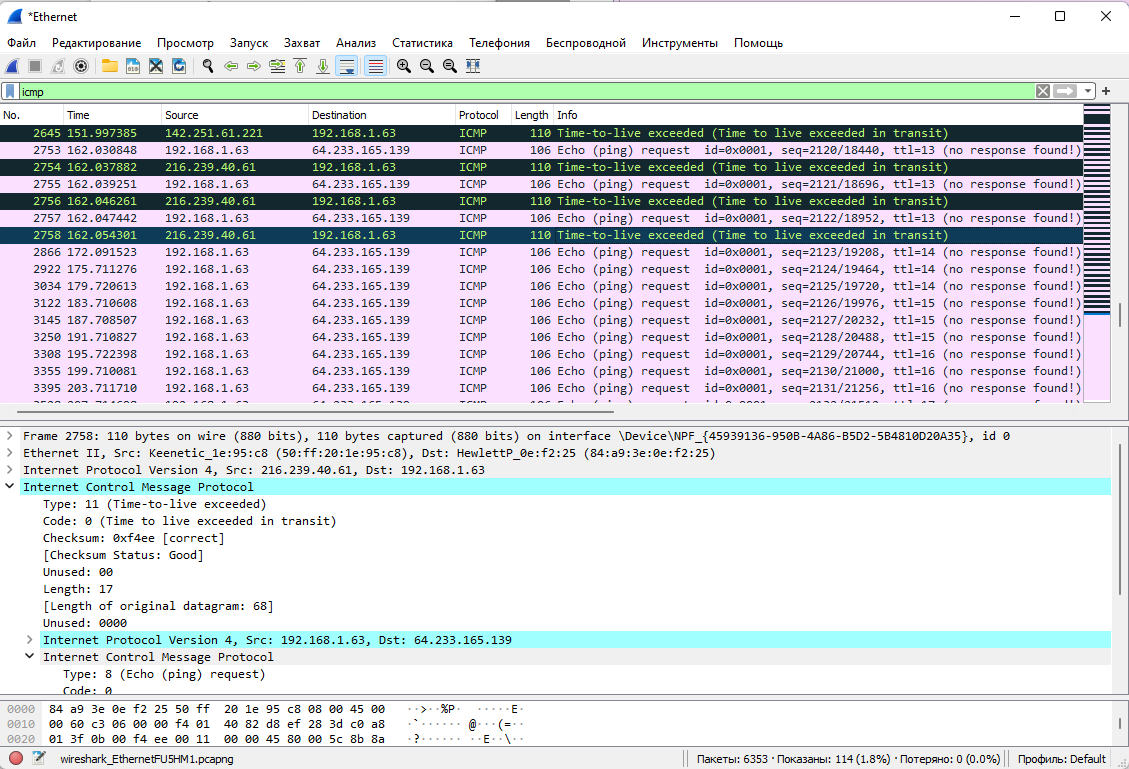
\includegraphics[width = 0.95\textwidth]{screenshots/5.png}}
\label{fig:image}
\end{center}

\begin{center}
\center{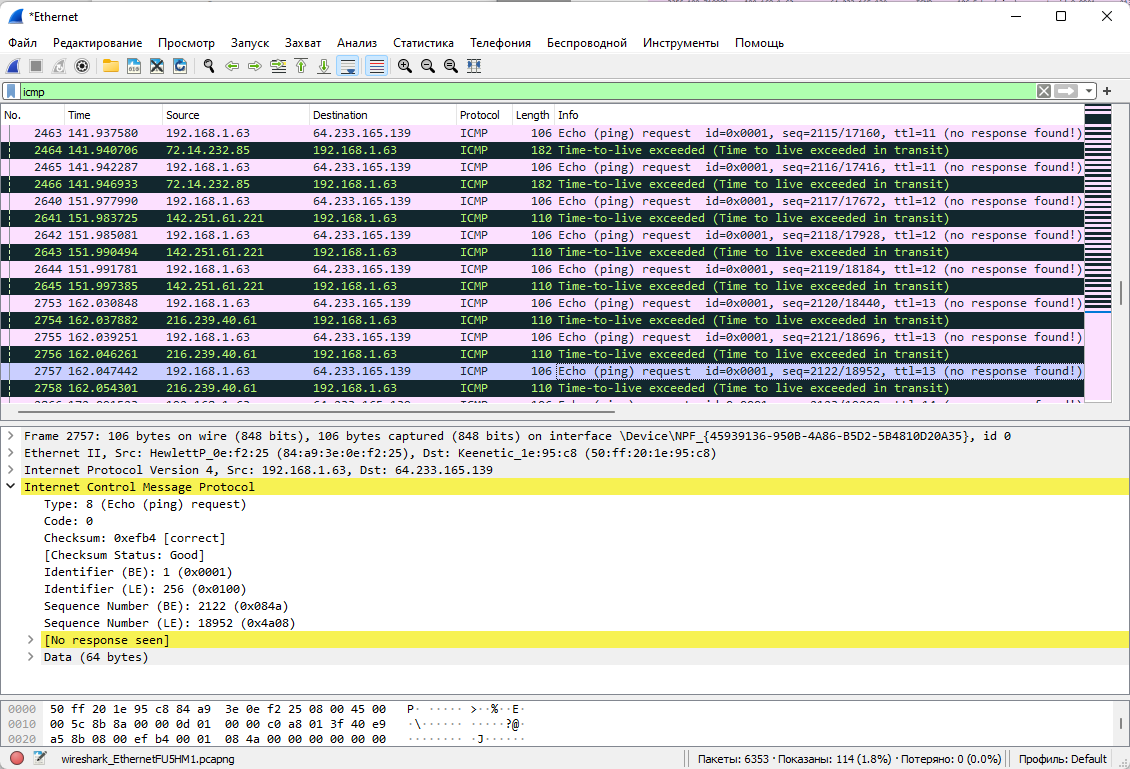
\includegraphics[width = 0.95\textwidth]{screenshots/7.png}}
\label{fig:image}
\end{center}
В пакете с ошибкой дополнительно есть поля: \\
Internet Protocol Version 4, Src: 192.168.1.63, Dst: 64.233.165.139 \\
Internet Control Message Protocol

3)
\begin{center}
\center{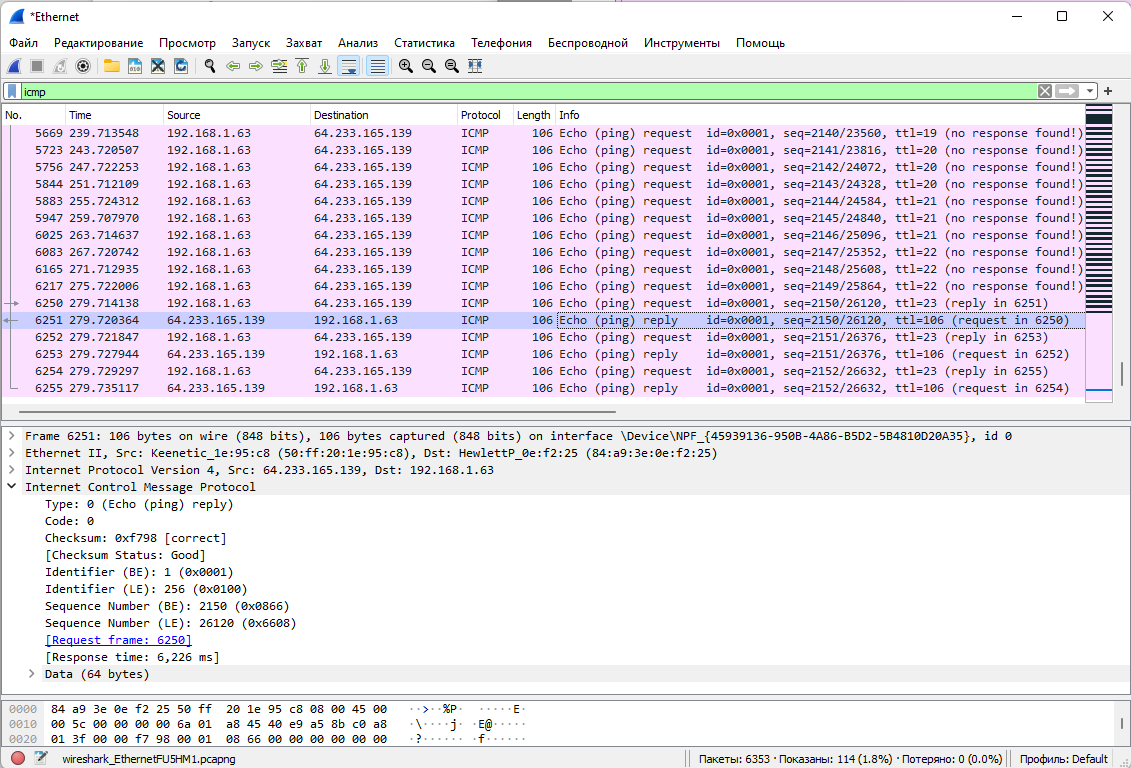
\includegraphics[width = \textwidth]{screenshots/6.png}}
\label{fig:image}
\end{center}
Type: 0 (Echo (ping) reply), нет дополнительных полей, которые были в пакетах с ошибками,  TTL = 106. Так произошло, так как последние пакеты успешно дошли до адреса и он ответил на запрос

\begin{center}
\center{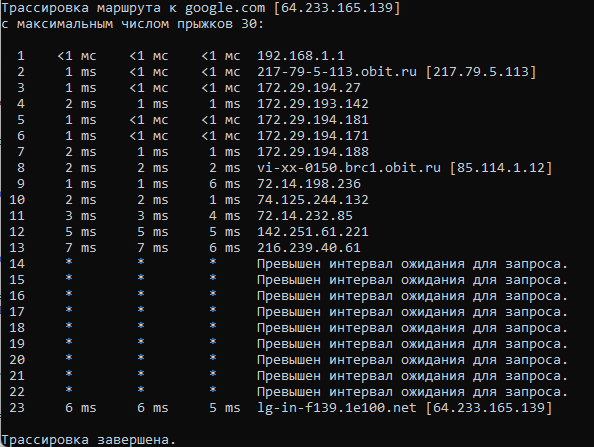
\includegraphics[width = \textwidth]{screenshots/8.png}}
\label{fig:image}
\end{center}
4) В данном случае оказалось так, что не было сильного отличия средней задержки, самая большая задержка была между 72.14.232.85 (Country: US) и 142.251.61.221 (Country: US)
\end{document}








































